\documentclass[a4paper,ngerman,12pt]{scrartcl}

\usepackage[utf8]{inputenc}
%\usepackage[ansinew]{inputenc}

\usepackage[ngerman]{babel}

\usepackage{amsmath,amsthm,amssymb,stmaryrd,color,graphicx}
\usepackage{setspace}
\usepackage{bussproofs}
\usepackage{array}
\usepackage{comment}

\usepackage{enumitem}

\usepackage{units}

\usepackage[protrusion=true,expansion=true]{microtype}

\usepackage{lmodern}

\usepackage{hyperref}
\usepackage{cleveref}

\newcommand{\RR}{\mathbb{R}}
\newcommand{\CC}{\mathbb{C}}
\newcommand{\ZZ}{\mathbb{Z}}
\newcommand{\NN}{\mathbb{N}}
\newcommand{\QQ}{\mathbb{Q}}

\setlength\parskip{\medskipamount}
\setlength\parindent{0pt}

\theoremstyle{definition}
\newtheorem{defn}{Definition}[]
\newtheorem{axiom}[defn]{Axiom}
\newtheorem{bsp}[defn]{Beispiel}

\theoremstyle{plain}
\newtheorem{prop}[defn]{Proposition}
\newtheorem{motto}[defn]{Motto}
\newtheorem{wunder}[defn]{Wunder}
\newtheorem{ueberlegung}[defn]{Überlegung}
\newtheorem{lemma}[defn]{Lemma}
\newtheorem{kor}[defn]{Korollar}
\newtheorem{hilfsaussage}[defn]{Hilfsaussage}
\newtheorem{satz}[defn]{Satz}

\theoremstyle{remark}
\newtheorem{bem}[defn]{Bemerkung}
\newtheorem{aufg}[defn]{Aufgabe}

\newlength{\aufgabenskip}
\setlength{\aufgabenskip}{1.4em}
\newcounter{aufgabennummer}
\newenvironment{aufgabe}[1]{
  \addtocounter{aufgabennummer}{1}
  \textbf{Aufgabe \theaufgabennummer.} \emph{#1} \par
}{\vspace{\aufgabenskip}}

\clubpenalty=10000
\widowpenalty=10000
\displaywidowpenalty=10000

\setlength\unitlength{1cm}

\usepackage{tikz}

\RequirePackage{geometry}
\geometry{textwidth=16.0cm,textheight=24.5cm,footskip=1.5cm}

\begin{document}

\begin{picture}(0,0)
  \put(0,-0.5){%
    
\includegraphics[scale=0.1]{logo-ifm}
  }
  \put(14.0,-3.5){%
    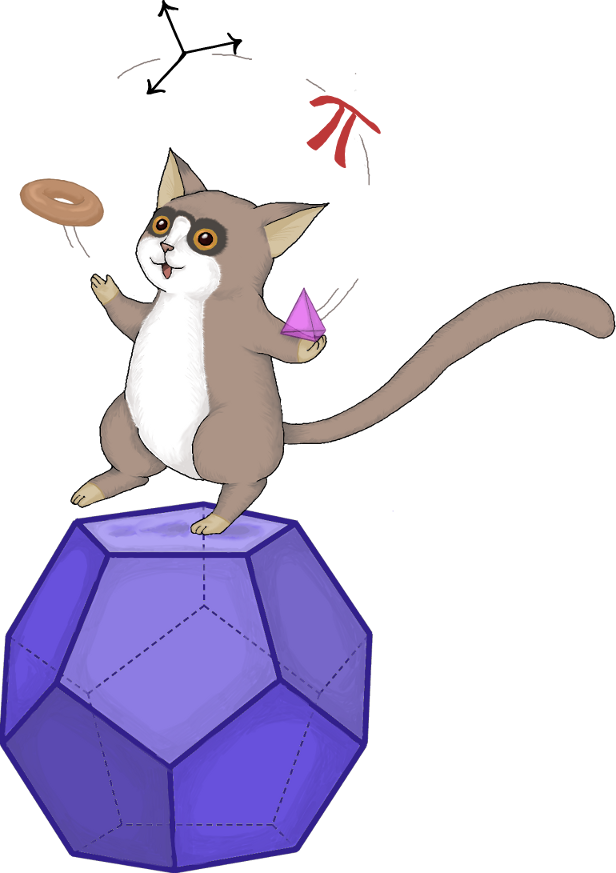
\includegraphics[scale=0.17]{cover}
  }
\end{picture} 

\vspace{6em}

\begin{center}\Large{Dritter Korrespondenzbrief}\end{center}

\section*{Fraktale Dimensionen}

Einleitung!


\section{Die Kochsche Schneeflocke}

Ersten zwei Schritte einer Konstruktion eines Musters:

\begin{center}
	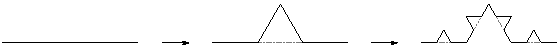
\includegraphics[width=.9\textwidth]{Bilder/Schneeflocke-Konstruktion1.pdf}
\end{center}

Wie du siehst, beginnt alles mit einer einfachen Strecke. Diese Strecke teilen wir in drei gleich lange Teile. Dann entfernen wir das mittlere Stück und ersetzen es durch die zwei anderen Seiten eines gleichseitigen Dreiecks. Dadurch erhalten wir eine geometrische Figur, die aus vier Strecken besteht. Für den zweiten Schritt machen wir nun mit jeder dieser vier Strecken das gleiche wie wir es mit der ersten Strecke getan haben.

Kannst du den dritten Schritt jetzt selbst zeichnen?

\begin{center}
	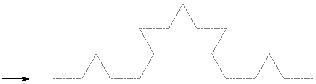
\includegraphics[width=.7\textwidth]{Bilder/Schneeflocke-Konstruktion2.pdf}
\end{center}

Wenn du möchtest kannst du auch noch einen vierten Schritt zeichnen. Schaffst du sogar einen fünften? Ziemlich bald wird es vermutlich schwierig noch weitere Schritte zu machen - einfach weil die Strecken so kurz werden, dass wir sie nicht mehr vernünftig teilen können. Aber zumindest vorstellen können wir uns doch, dass wir mit diesem Verfahren immer weiter machen - einen siebten Schritt, einen achten Schritt, usw. 

\begin{center}
	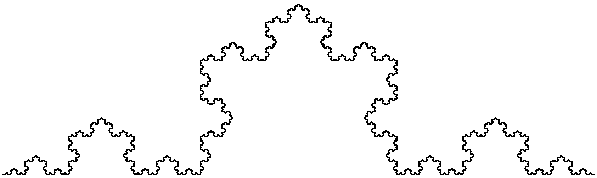
\includegraphics[width=.5\textwidth]{Bilder/Schneeflocke-Konstruktion3.pdf}
\end{center}

Tatsächlich wollen wir sogar \glqq unendlich viele\grqq{} Schritte machen und uns fragen, was für ein geometrisches Objekt wir dadurch erhalten. Dieses Objekt nennen wir dann \emph{die Kochsche Kurve}. Diese Kurve können wir natürlich nicht mehr zeichnen, aber wir können uns trotzdem überlegen, was für Eigenschaften sie haben muss. Und genau das wollen wir in diesem Brief tun. 

Als erstes wollen wir uns einmal überlegen, wie lang die Linie wohl sein muss, aus der die Kochsche Kurve \glqq nach unendlich vielen Schritten\grqq{} besteht. Da wir sie nicht zeichnen können, können wir natürlich nicht einfach nachmessen. Statt dessen wollen wir uns überlegen, was in einem einzelnen Schritt mit der Länge der Linie geschieht.

Dazu wollen wir annehmen, dass die Strecke ganz zu Beginn die Länge $l$ hat. Wie ist dann die Länge der Linie nach dem ersten Schritt? Nun, zuerst haben wir die Strecke in drei gleich lange Strecken geteilt und die mittlere davon entfernt - bleibt also noch eine Länge von $\frac{2}{3}l$. Dann haben wir in der Mitte zwei Seiten eines gleichseitigen Dreiecks gezeichnet, wobei jede der beiden Seiten so lang ist, wie die beiden Strecken. Also hat unsere gesamte Linie nach dem zweiten Schritt eine Länge von $\frac{2}{3}l + 2\cdot\frac{1}{3}l = \frac{4}{3}l$. Unsere neue Linie ist also $\frac{4}{3}$-mal so lang wie die ursprüngliche (miss in der Zeichnung doch einmal nach, ob das auch tatsächlich stimmt!).

Was passiert nun im zweiten Schritt? Unser Objekt besteht doch jetzt aus vier Strecken - und mit jeder von diesen machen wir das, was wir schon im ersten Schritt gemacht haben. Also wissen wir schon, dass jede dieser vier Strecken wieder $\frac{4}{3}$-mal so lang wird. Wenn wir nun aber jeden Teil der Linie $\frac{4}{3}$-mal so lang machen, dann machen wir damit auch das gesamte Objekt $\frac{4}{3}$-mal so lang. Folglich hat die Figur nach dem zweiten Schritt eine Länge von $\frac{4}{3}\cdot\frac{4}{3}l$. 

\begin{aufgabe}{}
	Wie lang ist die Figur dann nach dem dritten Schritt? Wie lang nach dem fünften? Nimm dir einen Moment Zeit darüber nachzudenken. Kannst du allgemein sagen, wie man ausrechnen kann, wie lang die Figur nach dem $n$-ten Schritt ist? 
\end{aufgabe}

Wie du sehen kannst, wird die Figur mit jedem Schritt länger - und das sogar mit jedem Schritt ein wenig schneller. Damit können wir endlich zu unserer Ausgangsfrage zurückkommen: Wie lang ist die Linie, aus der die Kochsche Kurve besteht?

\begin{satz}\label{satz:Kochkurve_laenge}
Die Kochsche Kurve ist unendlich lang.
\end{satz} 

\begin{proof}
Wir wollen zeigen, dass die Kurve unendlich lang ist - oder mit anderen Worten: Dass sie länger ist als jede endlich lange Kurve.

Sagen wir die Strecke ganz zu Beginn war \unit[3]{cm} lang. Ist die Kochsche Kurve dann länger als \unit[4]{cm}? Ja, ist sie - denn schon nach dem ersten Schritt ist die Kurve $\frac{4}{3}\cdot\unit[3]{cm} = \unit[4]{cm}$ lang. Und mit jedem weiteren Schritt wird sie nur noch länger. 

Ist sie auch länger als \unit[5]{cm}? Selbstverständlich, denn bereits nach dem zweiten Schritt ist die Kurve $\frac{4}{3}\cdot\unit[4]{cm} = \unit[\frac{16}{3}]{cm}\geq  \unit[5]{cm}$ lang. Ist sie auch länger als \unit[6]{cm}? Ja - und du siehst jetzt vermutlich schon selbst, warum das so ist. 

Tatsächlich können wir auf diese Weise sehen, dass die Kochsche Kurve länger als \emph{jede} endlich lange Kurve ist. Also ist sie \emph{unendlich} lang!
\end{proof}

Die Kochsche Kurve ist also eine \emph{unendlich lange Linie} - und das, obwohl sie einen Anfangs und einen Endpunkt hat (der linke und rechte Punkt der Figur wird ja in keinem Schritt verändert). Ein seltsames Objekt, nicht wahr? Und wie wir in diesem Brief sehen werden, ist sie nicht das einzige Objekt mit solch seltsamen Eigenschaften!

\begin{aufgabe}{Wo ist der Schnee?}
Vielleicht ist dir aufgefallen, dass die Überschrift dieses Kapitels \glqq Kochsche Schneeflocke\grqq{} lautet - bisher ist in diesem Kapitel aber keine Schneeflocke aufgetaucht. Wo hat sie sich also versteckt? Nun in gewisser Weise in folgendem Bild:
	\begin{center}
		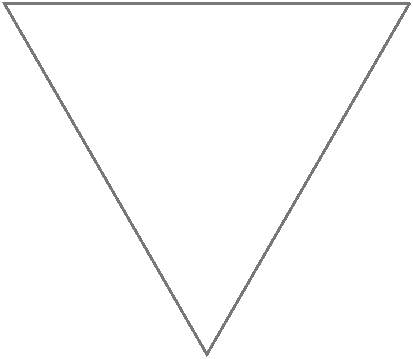
\includegraphics[width=.6\textwidth]{Bilder/Eigene_Schneeflocke.pdf}
	\end{center}	
Na gut, eine richtige Schneeflocke ist das noch nicht. Aber du kannst ganz leicht eine daraus machen! Fasse einfach jede der drei Seiten des obigen Dreiecks als Anfangsstrecke für eine Kochsche Kurve auf und führe mit jeder der drei Seiten zwei, drei Schritte der obigen Konstruktion durch. Siehst du jetzt eine Schneeflocke?

Das Objekt, dass man theoretisch \glqq nach unendlich vielen Schritten\grqq{} bekommen würde, nennt man auch \emph{Kochsche Schneeflocke}. Es besteht aus drei zusammengeklebten Kochschen Kurven. Damit können wir schon direkt sagen, wie lang der Umfang der Kochschen Schneeflocke ist - nämlich:

Eine etwas schwerere Zusatzaufgabe besteht darin, sich zu überlegen wie groß die Fläche innerhalb dieser Schneeflocke ist. Den genauen Flächeninhalt zu berechnen, ist vielleicht ein wenig schwierig (aber vielleicht hast du ja trotzdem eine Idee?). Deutlich einfacher ist es den Flächeninhalt nur grob zu schätzen: Ist er unendlich groß (wie der Umfang)? Oder ist er endlich groß? Kannst du deine Antwort begründen? Kannst du den Flächeninhalt irgendwie abschätzen (also zum Beispiel ein einfaches geometrisches Objekt angeben, das einen größeren Flächeninhalt hat - oder eine Zahl, die sicher größer ist als der Flächeninhalt der Schneeflocke\footnote{Dabei kannst du der Einfachheit annehmen, dass das ursprüngliche Dreieck eine Seitenlänge von $1$ und damit eine Höhe von $\frac{\sqrt{3}}{2}$ hat.} ).
\end{aufgabe}


\section{Dimensionen}

Wie wir im vorherigen Kapitel gesehen haben, sieht die Kochsche Kurve zwar aus wie eine Linie, sie verhält sich aber irgendwie nicht so wie wir das von einer normalen Linie erwarten würden. Dieses \glqq irgendwie\grqq{} wollen wir nun etwas genauer untersuchen:

Betrachte dazu zunächst eine ganz normale Strecke. Diese Strecke hat eine bestimmte Länge $l$. Was passiert, wenn wir diese Strecke um den Faktor $2$ strecken? Wie lang ist dann die neue Strecke? Na, $2l$, natürlich, denkst du jetzt vermutlich. Und selbstverständlich hast du auch recht. Aber um ganz sicher zu gehen, wollen wir das noch kurz beweisen.

\begin{center}
	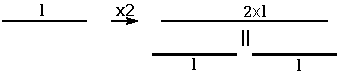
\includegraphics[width=.5\textwidth]{Bilder/Linie_vergroessern.pdf}
\end{center}

Und tatsächlich: Wie beginnen mit einer Strecke, strecken sie um den Faktor $2$ und erhalten eine neue Strecke, in die die alte genau zweimal hineinpasst. Die neue Strecke ist also tatsächlich zweimal so lang wie die alte.

Was passiert, wenn wir die Strecke um den Faktor $3$ strecken?
\begin{center}
	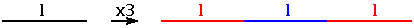
\includegraphics[width=.7\textwidth]{Bilder/Linie_vergroessern2.pdf}
\end{center}
Genau, sie wird dreimal so lang - d.h. zu einer Strecke, in die die alte Strecke dreimal hineinpasst. Keine Überraschungen soweit!

Also schauen wir doch mal, was mit unserer Kochschen Kurve passiert. Natürlich können wir hier nicht mehr wirklich über deren Länge reden (wir haben ja schon festgestellt, dass sie unendlich lang ist). Aber wir können uns trotzdem überlegen, wie oft eine Kochsche Kurve in eine andere, um den Faktor $3$ gestreckte Kurve passt:
\begin{center}
	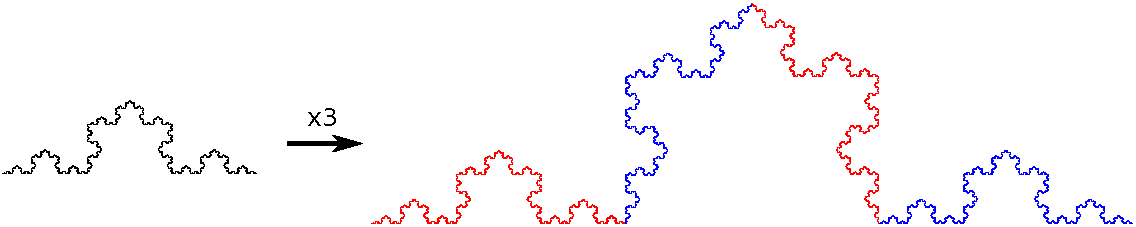
\includegraphics[width=.7\textwidth]{Bilder/KochKurve_vergroessern.pdf}
\end{center}
Na sowas! Wir haben die Kochsche Kurve um den Faktor $3$ gestreckt und auf einmal passt die alte Koch-Kurve \emph{viermal} in die neue (anstatt nur \emph{dreimal} wie wir das von der Linie gewohnt waren). In einem gewissen Sinne wird die Kochsche Kurve beim Strecken also \glqq schneller groß\grqq{} als eine gewöhnliche Linie.

Also suchen wir zum Vergleich mal nach anderen geometrischen Objekten, die beim Strecken schneller größer werden als eine Linie. Wie wäre es zum Beispiel mit dem Flächeninhalt eines Dreiecks? Wie oft passt ein Dreieck in ein um den Faktor $2$ gestrecktes Dreieck? Wie oft in ein um den Faktor $3$ gestrecktes Dreieck?
\begin{center}
	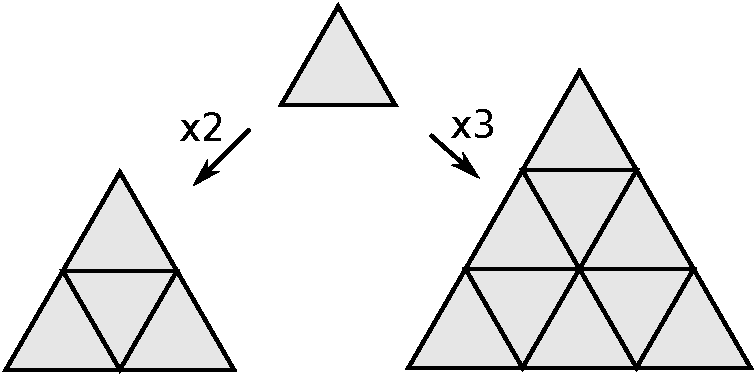
\includegraphics[width=.4\textwidth]{Bilder/Dreieck_vergroessern.pdf}
\end{center}
Offenbar viermal in ein zweimal so großes Dreieck und gleich neunmal in ein nur dreimal so großes Dreieck. Der Flächeninhalt eines Dreiecks wird also tatsächlich schneller größer als die Länge einer Linie. Und er wird sogar schneller größer als die Kochsche Kurve. Auf eine gewisse Weise scheint die Kochsche Kurve also irgendetwas zwischen einer Linie und einem Dreieck zu sein.

\begin{aufgabe}{Wie oft?}\label{aufgabe:Wie_oft}
Um das näher zu untersuchen wollen wir uns einmal eine Tabelle mit verschiedenen geometrischen Objekten anlegen und jeweils untersuchen, wie oft das ursprüngliche Objekt in eine $2$-fach, $3$-fach, $4$-fach und $9$-fach gestreckte Version davon passt:
\begin{center}
	\renewcommand{\arraystretch}{2}
	\begin{tabular}{l||c|c|c|c}
		Streckfaktor:& $2$-fach & $3$-fach & $4$-fach & $9$-fach \\\hline\hline
		Strecke      & $2$-mal	& $3$-mal  &          &			 \\\hline
		Dreieck      & $4$-mal  & $9$-mal  &          &          \\\hline
		Quadrat      &          &          &          &          \\\hline
		Würfel       &          &          &          &          \\\hline
		Kochschee Kurve & ---   & $4$-mal  & ---      &          \\      	
	\end{tabular}
\end{center}
Kannst du die noch fehlenden Einträge einfügen? Evtl. sind dabei Skizzen hilfreich (bzw. für den Würfel würfelförmige Bauklötze/Legosteine/o.ä.)
\end{aufgabe}

\begin{aufgabe}{Potenzen und Dimensionen}
Und dann hätte ich da noch eine Tabelle, die es auszufüllen gilt:
\begin{center}
	\renewcommand{\arraystretch}{2}
	\begin{tabular}{l||c|c|c|c}
				      & $2$ & $3$ & $4$ & $9$ \\\hline\hline
		$\boxed{\phantom{1}}^1$  & $2^1=2$	&   &  & \\\hline
		$\boxed{\phantom{1}}^2$  & $2^2=4$	& $3^2=9$ & \phantom{$4^2=16$} & \phantom{$9^2=81$}\\\hline
		$\boxed{\phantom{1}}^3$  & 	&   &  & \\\hline
		$\boxed{\phantom{1}}^{1,262}$  & 	&   &  &     	
	\end{tabular}
\end{center}
(für die letzte Zeile brauchst du vermutlich einen Taschenrechner - wenn du gerade keinen zur Hand hast, der soetwas berechnen kann, kannst du auch einfach grob schätzen, wie groß die entsprechende Zahl wohl sein müsste (z.B. größer als $3$ aber kleiner als $9$)).

Wenn du beide Tabellen fertig ausgefüllt hast, vergleiche einmal die verschiedenen Einträge miteinander. Fällt dir etwas auf?

\emph{Tipp:} Strecken sind eindimensionale Objekte, Flächen sind zweidimensionale Objekte und Volumen sind dreidimensional.\footnote{Zusatzfrage: Punkte bezeichnet man oft als 0-dimensionale Objekte - wie passt das in dieses Schema?}
\end{aufgabe}

\begin{defn}
Streckt man ein geometrisches Objekt um den Streckungsfaktor $k$ und das ursprüngliche Objekt passt dann $k^d$-mal in das ursprüngliche Objekt, so sagen wir: Das Objekt hat die \emph{Dimension $d$}.\footnote{Tatsächlich gibt es mehrere Möglichkeiten fraktale Dimensionen zu definieren - wir betrachten hier die sogenannte \glqq Ähnlichkeits-Dimension\grqq{}}

Ist dieses $d$ keine ganze Zahl, so nennen wir diese Dimension \emph{fraktale Dimension} und das geometrische Objekt nennen wir ein \emph{Fraktal}.
\end{defn}

\begin{bem}
Die Kochsche Kurve ist also unser erstes Beispiel für ein solches Fraktal. Seine fraktale Dimension ist ungefähr $1,262$ - was gut zu unserer eingangs aufgestellten Vermutung passt, dass die Kochsche Kurve \emph{irgendetwas} zwischen einem eindimensionalen Objekt (wie einer Strecke) und einem zweidimensionalen (wie einem Dreieck) ist.
\end{bem}

\begin{bem}
Angenommen wir untersuchen ein geometrisches Objekt und wollen dessen Dimension bestimmen. Wir haben es also um den Faktor $k$ gestreckt und festgestellt, dass das ursprüngliche Objekt nun $n$-mal in das neue hineinpasst. Wie können wir jetzt herausfinden, was die Dimension ist? Wie finden wir also ein $d$ mit $k^d = n$?

Dazu gibt es die sogenannte \emph{Logarithmusfunktion} $\log_{\boxed{}}\boxed{\phantom{k}}$: Für zwei Zahlen $n$ und $k$ ist $\log_k n$ gerade die Zahl mit der wir $k$ potenzieren müssen um $n$ zu erhalten - d.h. $k^{\log_k n} = n$. Also ist $\log_k n$ gerade die Zahl, die auch unser $d$ sein soll. Wenn du einen Taschenrechner mit einer entsprechenden Funktion hast, kannst du das ja mal testen, indem du die fraktale Dimension der Kochschen Kurve nachrechnest.

Wenn du gerade keinen solchen Taschenrechner zur Hand hast, genügt es für das weitere Blatt aber auch, eine grobe Schätzung für $d$ zu finden. Zum Beispiel haben wir ja bereits herausgefunden, dass bei der Kochschen Kurve gilt: $3^d=4$ (in eine um den Faktor $3$ gestreckte Kochsche Kruve passt die ursprüngliche $4$-mal hinein). Jetzt können wir abschätzen:
\[3^1 = 3 < 4 = 3^d = 4 < 9 = 3^2\]
Also muss die fraktale Dimension der Kochschen Kurve irgendwo zwischen $1$ und $2$ liegen.
\end{bem}

\section{Mehr Fraktale}

Nachdem du nun das notwendige Handwerkszeug besitzt um Fraktale zu untersuchen, hast du in diesem Kapitel nun die Gelegenheit dazu:

\subsection{Ein Fraktal-Baum}

Unser erstes Fraktal entsteht durch folgende Konstruktionsregel:
\begin{center}
	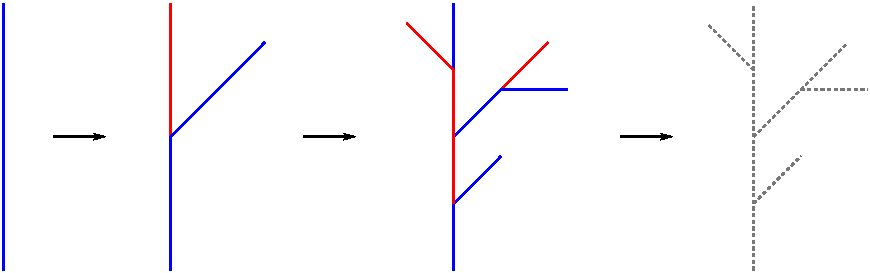
\includegraphics[width=.7\textwidth]{Bilder/Baum-Konstruktion.pdf}
\end{center}


\begin{aufgabe}{}
	Wie du sehen kannst, kommen bei der Konstruktion dieses Fraktals Strecken in zwei verschiedenen Farben vor. Die beiden Farben haben jeweils leicht unterschiedliche Ersetzungsregeln. Kannst du diese aus den ersten beiden Schritten erkennen und den Baum im dritten Schritt fertig zeichnen? 
	
	Kannst du außerdem die fraktale Dimension dieses Baumes bestimmen? Dazu kannst du zum Beispiel versuchen wieder eine Tabelle wie in \Cref{aufgabe:Wie_oft} auszufüllen\footnote{Beim Bestimmen der Ähnlichkeitsdimension kannst du die verschiedenen Farben der Äste ignorieren - diese dienen nur als Hilfe für die Konstruktion.}:
	\begin{center}
		\renewcommand{\arraystretch}{2}
		\begin{tabular}{l||c|c|c|c}
			Streckfaktor:& $2$-fach & $3$-fach & $4$-fach & $9$-fach \\\hline\hline
			Fraktal-Baum & 	&   &          &			 \\	
		\end{tabular}
	\end{center}
\end{aufgabe}


\subsection{Das Sierpinski-Dreieck}

Es gibt aber nicht nur Fraktale aus Linien - man kann genauso gut Fraktale aus zweidimensionalen Objekten bauen. Zum Beispiel so:
\begin{center}
	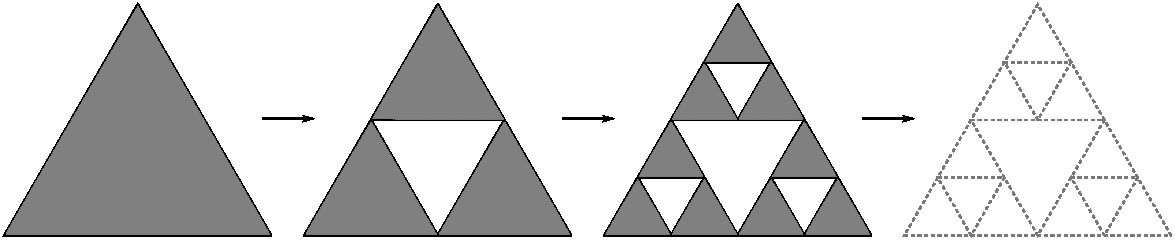
\includegraphics[width=.7\textwidth]{Bilder/Sierpinski-Konstruktion.pdf}
\end{center}

\begin{aufgabe}{}\label{aufgabe:Sierpinski-Flaeche}
	Wir beginnen diesmal also mit einem grauen gleichseitigen Dreieck. Für den ersten Schritt schneiden wir daraus ein umgekehrtes gleichsetiges Dreieck aus und erhalten so eine neue Figur aus drei grauen und einem weißen Dreieck. Für den zweiten Schritt geht es mit den drei grauen Dreiecken so weiter wie im ersten Schritt. Kannst du die Figur nach dem dritten Schritt zeichnen?
	
	Die Figur, die man erhält, wenn man unendlich viele solche Schritte macht, heißt \emph{Sierpinski-Dreieck} und ist wieder ein Fraktal. Kannst du dessen Dimension bestimmen?
\end{aufgabe}

\begin{aufgabe}{}
	Kannst du die (graue) Fläche des Sierpinski-Dreiecks bestimmen? 
	
	Du kannst dazu analog zum Beweis von \Cref{satz:Kochkurve_laenge} vorgehen: Wenn das ursprüngliche Dreieck eine Fläche von $\unit[4]{cm^2}$ hat. Welche (graue) Fläche hat man dann nach dem ersten Schritt? Und nach dem zweiten? Nach $n$ Schritten? Gibt es irgendeine Zahl, von der du sicher sagen, kannst, dass das Sierpinksi Dreieck einen größeren Flächeninhalt hat, als diese Zahl?
\end{aufgabe}

\begin{aufgabe}{Pascalsches Dreieck}
	Erinnerst du dich noch an das Pascalsche Dreieck aus dem ersten Korrespondenzbrief? (falls nicht, schau einfach kurz nach - er kam in Aufgabe 4 vor)
	
	Befülle dann die folgende Figur so mit Zahlen, dass das Pascalsche Dreieck entsteht (in jedem der Sechsecke soll also eine Zahl stehen und in jeder Zeile steht im linken und im rechten Sechseck eine $1$):
	\begin{center}
			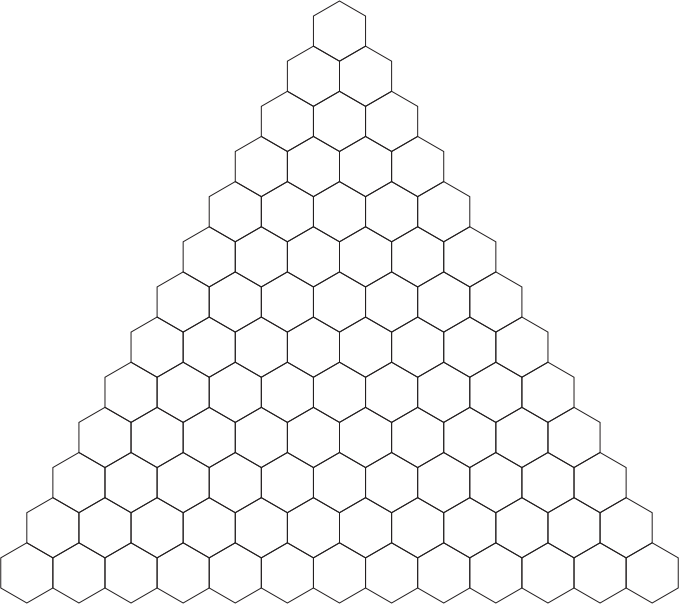
\includegraphics{Bilder/pascal-triangle.png}
	\end{center}
	Wenn du das gemacht hast, male alle Sechsecke aus, in denen eine ungerade Zahl steht. Fällt dir dabei etwas auf?
\end{aufgabe}


\subsection{Die Cantor-Menge}\label{aufgabe:Cantor-Menge}

Ein eng zum Sierpinski-Dreieck verwandtes Fraktal ist die \emph{Cantor-Menge}. Dazu starten wir mit einer einfachen Strecke und entfernen das mittlere Drittel dieser Strecke. Dadurch erhalten wir zwei Strecken, von denen wir wiederum jeweils das mittlere Drittel entfernen usw.

\begin{center}
	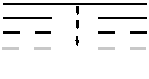
\includegraphics[width=.7\textwidth]{Bilder/Cantor_Menge.pdf}
\end{center}

\begin{aufgabe}{}
	Zeichne den nächsten und übernächsten Schritt in der Konstruktion der Cantor-Menge. Bestimme die fraktale Dimension der Cantor-Menge. 
	
	Kannst du auch die Gesamtlänge aller \glqq Streckenstücke\grqq bestimmen, aus der die Cantor-Menge besteht? (du kannst dazu wieder analog zu \Cref{satz:Kochkurve_laenge} und \Cref{aufgabe:Sierpinski-Flaeche} vorgehen).
\end{aufgabe}


\subsection{Pyramiden-Fraktal}

Kann man eigentlich auch aus dreidimensionalen Objekten Fraktale bauen? Aber selbstverständlich kann man das - man braucht nur etwas mehr Vorstellungskraft:

\begin{center}
	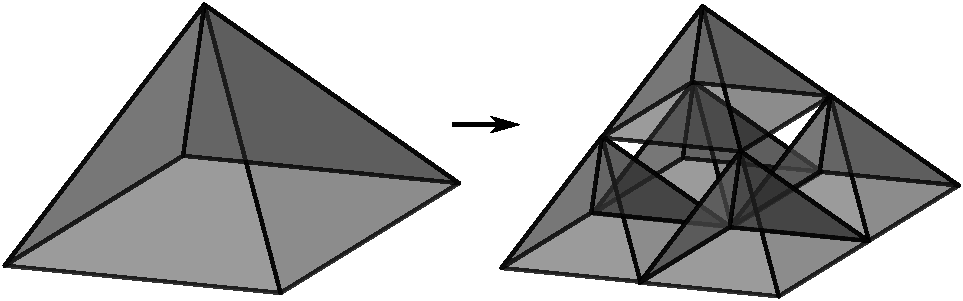
\includegraphics[width=.6\textwidth]{Bilder/Pyramiden.pdf}
\end{center}

\begin{aufgabe}{}
	Wie du siehst, starten wir diesmal mit einer Pyramide und ersetzen diese dann im ersten Schritt durch fünf kleinere Pyramiden. Im zweiten Schritt müssten wir dann jede dieser Pyramiden wieder durch fünf noch kleinere ersetzen. Wie viele Pyramiden haben wir also nach dem zweiten Schritt? (wenn du möchtest, kannst auch mal versuchen zu zeichnen, wie das nach dem zweiten Schritt aussieht - ich fürchte allerdings, dass das ziemlich unübersichtlich wird).
	
	Kannst du die fraktale Dimension dieses Objektes bestimmen? 
	
	Kannst du mit Hilfe der fraktalen Dimension erraten,  wie groß wohl Volumen und Oberfläche dieses Fraktals sein werden? (vergleiche dazu deine entsprechenden Ergebnisse zur Kochschen Kurve, dem Sierpinski-Dreieck und der Cantor-Menge) 
	
	Wenn du bereits die Volumen- bzw. Oberflächenformel für Pyramiden kennst, kannst Volumen und Oberfläche des Pyramidenfraktals natürlich auch wieder direkt bestimmen (wie bei der Kochkurve, dem Sierpinski-Dreieck und der Cantor-Menge).
\end{aufgabe}
 
%\subsection{Drachenkurve}
%
%\begin{center}
%	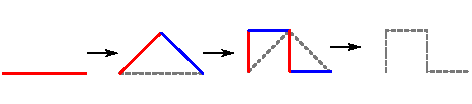
\includegraphics[width=.7\textwidth]{Bilder/Drachenkurve_Konstruktion.pdf}
%\end{center}

%\begin{aufgabe}{Ein gebasteltes Fraktal}
%	Inhalt...
%\end{aufgabe}

\subsection{Noch ein Fraktal?}

\begin{center}
	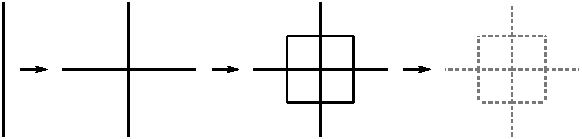
\includegraphics{Bilder/Nicht-Fraktal.pdf}
\end{center}

\begin{aufgabe}{}
	Zeichne den nächsten Schritt in dieser Konstruktion und bestimme dann die fraktale Dimension dieses Objekts.
	
	Kannst du dir vorstellen, was es bedeutet, dass das Objekt diese Dimension hat?
\end{aufgabe}

\subsection{Wie lang ist Deutschland Küste?}

Beim Recherchieren für diesen Korrespondenzbrief habe ich immer wieder gelesen, dass Fraktale nicht nur eine abstrakte mathematische Idee seinen. Vielmehr treten Frakale oder zumindest fraktalartige Dinge angeblich auch in der Natur auf. Und eines der häufigsten Beispiele dafür sind Meeresküsten - wie zum Beispiel die deutsche Nordsee-Küste - die du hier in drei verschiedenen Maßstäben abgebildet siehst:

TODO: Bild einfügen!

\begin{aufgabe}
Zum Abschluss dieses Briefes wollen wir jetzt also nachprüfen, ob man wirklich sagen kann, dass die deutsche Küste \glqq frakalartige Eigenschaften\grqq hat. 

Wenn du dir die obigen Bilder anschaust, kannst du vielleicht schon eine erste Ähnlichkeit zu unseren bisherigen Fraktalen erkennen: Je näher man an die Küstenlinie heranzoomt, desto mehr Zacken und Einbuchtungen kann man erkennen (so wie zum Beispiel auch bei der Kochschen Kurve). Gleichzeitig siehst du aber vermutlich auch, dass diese Küstenlinie nicht mit Hilfe einer so einfachen Konstruktionsvorschrift gezeichnet werden kann, wie das bei den bisherigen Fraktalen der Fall war.

Daher können wir auch nicht so einfach die frakale Dimension bestimmen wie das bisher der Fall war.\footnote{Es geht trotzdem - dafür bräuchten wir aber eine etwas andere Definition von Dimension.} Zumindest aber können wir versuchen ungefähr abzuschätzen, was die fraktale Dimension der Küstenlinie sein sollte - insbesondere also, ob sie eine ganze Zahl ist oder nicht.

Dafür werden wir gleich versuchen die Länge der Küstenlinie zu messen. Bevor du das machst, versuche folgende Fragen zu beantworten: Aufgrund deiner bisherigen Erfahrungen mit Fraktalen: Welche Länge sollte die Küste haben, wenn sie eine Dimension kleiner als $1$ hat? Welche Länge, wenn sie eine Dimension größer als $1$ hat? Und was wäre, wenn sie genau Dimension $1$ hätte (also überhaupt kein Fraktal wäre)?

Um die Länge der Küste zu messen, wollen wir wie folgt vorgehen: Zunächst wollen wir nur ganz grob die Länge bestimmen - dazu messen wir die Länge im größten Maßstab. Dann die im nächstgrößeren Maßstab. Und schließlich die im größten Maßstab. Trage deine Ergebnisse in der folgenden Tabelle ein:

TODO: Tabelle einfügen 

\emph{Tipp:} Am leichtesten kannst du die Küstenlänge messen, indem du einen Faden entlang der Küste legst und dann dessen Länge misst.

Kannst du in der Tabelle ein Muster erkennen? Angenommen dieses Muster setzt sich auch bei weiteren, immer genaueren Messungen so fort - was würde dann wohl die tatsächliche Länge der deutschen Küste sein? Was kannst du damit über deren fraktale Dimension aussagen?
\end{aufgabe}

\end{document}
